\documentclass[11pt]{article}
\usepackage{times}
\usepackage[cm]{fullpage}
\usepackage{amsmath,amssymb}
\usepackage{booktabs}
\usepackage{tabularx}
\newcolumntype{Y}{>{\raggedright\arraybackslash}X}
\usepackage{enumitem}
\usepackage{xcolor}
\usepackage{hyperref}
\usepackage{microtype}
\usepackage{tikz}
\usetikzlibrary{arrows.meta,positioning,fit,backgrounds,calc,shapes.geometric}
\hypersetup{hidelinks}

\definecolor{primitivecol}{RGB}{85,85,85}
\definecolor{optioncol}{RGB}{183,83,42}
\definecolor{landmarkcol}{RGB}{42,104,155}
\definecolor{goalcol}{RGB}{34,120,52}
\definecolor{actR}{RGB}{220,50,40}
\definecolor{actC}{RGB}{30,170,170}
\definecolor{actO}{RGB}{235,150,30}

\tikzset{
  pgm latent/.style={circle,draw,minimum size=9mm,inner sep=1pt,font=\small},
  pgm observed/.style={circle,draw,fill=black!15,minimum size=9mm,inner sep=1pt,font=\small},
  pgm parameter/.style={rectangle,draw,rounded corners=1pt,minimum height=7mm,inner sep=3pt,font=\small},
  pgm map/.style={diamond,draw,fill=landmarkcol!10,aspect=1.8,inner sep=2pt,font=\small},
  pgm arrow/.style={-{Stealth[length=3pt]},line width=0.75pt},
  pgm plate/.style={draw,rounded corners,inner sep=5pt},
  gcell/.style={draw,rounded corners=1pt,minimum size=9mm,inner sep=1pt,font=\small},
  lcell/.style={gcell,fill=landmarkcol!18,draw=landmarkcol,line width=1pt}
}

\title{How to Abstract a Problem-Solving Task?\\
\large Analysis 7: The Generative Model of Cognitive Maps and Search}
\author{}
\date{7 June 2026}

\begin{document}
\maketitle

\begin{abstract}
This note specifies one \emph{generative model} shared by three agent families: a
primitive planner, an action-chunk planner, and a landmark-option planner. Every family
stores a static, task-independent representation $\mathcal R_M$ that deterministically
induces a cognitive transition map $\mathcal K_M=F_M(\mathcal K_0,\mathcal R_M)$; a common
heuristic-search kernel selects transitions and a common execution model emits primitive
behavior. The abstraction is a \emph{hidden layer over observed primitives}: the chunk
family groups \emph{action} sequences into a grammar $\mathcal G$ (with a per-occurrence
parse $z^{g}$), while the landmark family groups \emph{states} into regions through a
static membership $z^{\ell}:\mathcal S\to\mathcal L$ with a directed region graph
$\mathcal E^{\mathcal L}$. We reserve $z$ for these latent assignments, describe the
trajectory's segmentation with a time-series change-point process $\chi$, and make the one
search distance $d^{*}$ explicit. Recovering the representation by Bayesian structural EM is
the companion Analysis 8.
\end{abstract}

\section{One hierarchy for all three agents}

Let the primitive task graph be $\mathcal K_0=(\mathcal S,\mathcal E_0,\omega_0)$, and let
trial $n$ contain the observed trajectory
\[
\tau_n=(s_{n,0},a_{n,1},s_{n,1},\ldots,a_{n,T_n},s_{n,T_n}),
\]
with goal $s_{\star,n}$. The candidate model space is
$\mathcal M=\{M_{\mathrm{primitive}},M_{\mathrm{option}},M_{\mathrm{landmark}}\}$, and all
families share one chain:
\begin{equation}
\boxed{
\;\mathcal R_M\ \longrightarrow\ \mathcal K_M=F_M(\mathcal K_0,\mathcal R_M)\ \longrightarrow\
z\ \longrightarrow\ \tau_n\;}.
\label{eq:hierarchy}
\end{equation}
Here $\mathcal R_M$ is the agent's stored, \emph{task-independent} knowledge; $\mathcal K_M$
is the map it induces; and $z$ is the latent assignment that lifts each observed primitive
to the hidden abstract layer. The boundaries of the resulting segments are summarized by a
separate time-series object $\chi$ (\S\ref{sec:hidden}); we reserve $z$ for the genuine
latent and never overload it with segmentation bookkeeping.

\section{The same data stream, two abstractions}
\label{sec:overview}

A single transition stream $\{(s_{n,t-1},a_{n,t},s_{n,t})\}$ can be read two ways. Reading
it as a sequence of \emph{actions} $\{a_t\}$ invites a grammar over action strings; reading
it as a sequence of \emph{states} $\{s_t\}$ invites a grouping of states into landmark
regions. This is the deepest difference between the families and the reason their
``primitive'' differs (Figure~\ref{fig:overview}).

\begin{figure}[htbp]
\centering
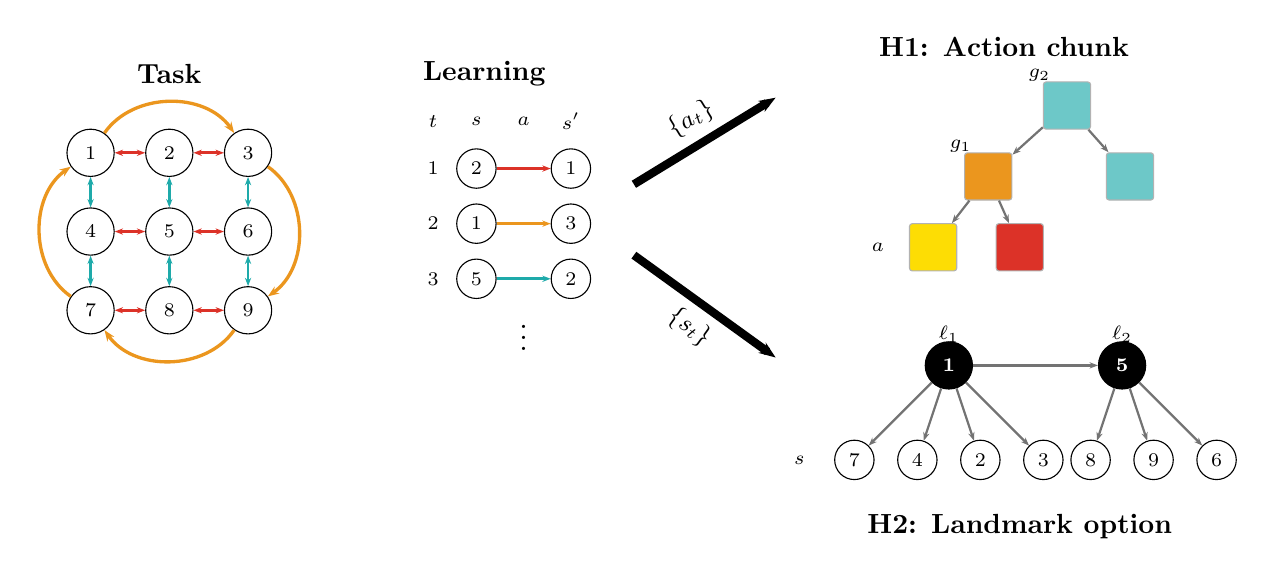
\begin{tikzpicture}[
  x=1cm,y=1cm,
  ts/.style={circle,draw,minimum size=6mm,inner sep=0pt,font=\scriptsize},
  lmk/.style={circle,draw,fill=black,text=white,minimum size=6mm,inner sep=0pt,font=\scriptsize\bfseries},
  redd/.style={{Stealth[length=3pt]}-{Stealth[length=3pt]},actR,line width=1pt},
  cyann/.style={{Stealth[length=3pt]}-{Stealth[length=3pt]},actC,line width=1pt},
  oran/.style={-{Stealth[length=4pt]},actO,line width=1.2pt},
  gry/.style={-{Stealth[length=3pt]},black!55,line width=0.8pt},
  blk/.style={-{Stealth[length=6pt]},line width=3pt},
  csq/.style={rectangle,rounded corners=1pt,minimum size=6mm,inner sep=0pt,draw=black!30}
]
  % ---------------- TASK ----------------
  \node[font=\bfseries] at (1,3) {Task};
  \foreach \id/\x/\y in {1/0/2,2/1/2,3/2/2,4/0/1,5/1/1,6/2/1,7/0/0,8/1/0,9/2/0}{
    \node[ts] (t\id) at (\x,\y) {\id};}
  \foreach \a/\b in {1/2,2/3,4/5,5/6,7/8,8/9}{\draw[redd] (t\a)--(t\b);}
  \foreach \a/\b in {1/4,4/7,2/5,5/8,3/6,6/9}{\draw[cyann] (t\a)--(t\b);}
  \draw[oran] (t1) to[bend left=55] (t3);
  \draw[oran] (t3) to[bend left=55] (t9);
  \draw[oran] (t9) to[bend left=55] (t7);
  \draw[oran] (t7) to[bend left=55] (t1);
  % ---------------- LEARNING ----------------
  \node[font=\bfseries] at (5,3) {Learning};
  \node[font=\scriptsize] at (4.35,2.4){$t$};\node[font=\scriptsize] at (4.9,2.4){$s$};
  \node[font=\scriptsize] at (5.5,2.4){$a$};\node[font=\scriptsize] at (6.1,2.4){$s'$};
  \node[font=\scriptsize] at (4.35,1.8){1};
  \node[ts,minimum size=5mm](r1s) at (4.9,1.8){2};\node[ts,minimum size=5mm](r1e) at (6.1,1.8){1};
  \draw[-{Stealth[length=3pt]},actR,line width=1pt] (r1s)--(r1e);
  \node[font=\scriptsize] at (4.35,1.1){2};
  \node[ts,minimum size=5mm](r2s) at (4.9,1.1){1};\node[ts,minimum size=5mm](r2e) at (6.1,1.1){3};
  \draw[-{Stealth[length=3pt]},actO,line width=1pt] (r2s)--(r2e);
  \node[font=\scriptsize] at (4.35,0.4){3};
  \node[ts,minimum size=5mm](r3s) at (4.9,0.4){5};\node[ts,minimum size=5mm](r3e) at (6.1,0.4){2};
  \draw[-{Stealth[length=3pt]},actC,line width=1pt] (r3s)--(r3e);
  \node[font=\large] at (5.5,-0.25){$\vdots$};
  % ---------------- SPLIT ARROWS ----------------
  \draw[blk] (6.9,1.6) -- (8.7,2.7) node[midway,above,sloped,font=\small]{$\{a_t\}$};
  \draw[blk] (6.9,0.7) -- (8.7,-0.6) node[midway,below,sloped,font=\small]{$\{s_t\}$};
  % ---------------- H1 chunk ----------------
  \node[font=\bfseries] at (11.6,3.35) {H1: Action chunk};
  \node[csq,fill=actC!65] (g2) at (12.4,2.6) {};
  \node[font=\scriptsize] at (12.05,2.98) {$g_2$};
  \node[csq,fill=actO] (g1) at (11.4,1.7) {};
  \node[font=\scriptsize] at (11.05,2.08) {$g_1$};
  \node[csq,fill=actC!65] (h3) at (13.2,1.7) {};
  \node[csq,fill=yellow!80!orange] (h1) at (10.7,0.8) {};
  \node[csq,fill=actR] (h2) at (11.8,0.8) {};
  \node[font=\scriptsize] at (10.0,0.8) {$a$};
  \draw[gry] (g2)--(g1); \draw[gry] (g2)--(h3);
  \draw[gry] (g1)--(h1); \draw[gry] (g1)--(h2);
  % ---------------- H2 landmark ----------------
  \node[font=\bfseries] at (11.8,-2.75) {H2: Landmark option};
  \node[lmk] (l1) at (10.9,-0.7) {1};
  \node[lmk] (l2) at (13.1,-0.7) {5};
  \node[font=\scriptsize] at (10.9,-0.3) {$\ell_1$};
  \node[font=\scriptsize] at (13.1,-0.3) {$\ell_2$};
  \draw[gry] (l1)--(l2);
  \foreach \id/\x in {7/9.7,4/10.5,2/11.3,3/12.1}{
    \node[ts,minimum size=5mm](b\id) at (\x,-1.9){\id}; \draw[gry] (l1)--(b\id);}
  \foreach \id/\x in {8/12.7,9/13.5,6/14.3}{
    \node[ts,minimum size=5mm](b\id) at (\x,-1.9){\id}; \draw[gry] (l2)--(b\id);}
  \node[font=\scriptsize] at (9.0,-1.9) {$s$};
\end{tikzpicture}
\caption{One environment, one data stream, two static abstractions. \emph{Task}: the
$3\times3$ graph with typed edges --- horizontal (red), vertical (cyan), and wrap-around
loop (orange). \emph{Learning}: the observed transitions $\{(s,a,s')\}$, each action coloured
by type. Reading the stream as actions $\{a_t\}$ yields \emph{H1}, an action-chunk grammar:
terminals are actions (coloured squares), the hidden non-terminals $g_1,g_2$ are the grammar
$\mathcal G$, and the per-occurrence parse is $z^{g}$. Reading it as states $\{s_t\}$ yields
\emph{H2}, a landmark partition: each observed state is assigned to a landmark by the static
hidden membership $z^{\ell}$, and the directed link $\ell_1\!\to\!\ell_2$ is the region
structure $\mathcal E^{\mathcal L}$. The chunk abstracts \emph{edges} (action sequences);
the landmark abstracts \emph{nodes} (the state set).}
\label{fig:overview}
\end{figure}

This node-versus-edge duality has a precise consequence. The state set $\mathcal S$ is a
fixed finite domain, so its abstraction can be a \emph{static set partition}: the landmark
membership $z^{\ell}:\mathcal S\to\mathcal L$ assigns each state, once and for all, to a
landmark region. Actions only acquire meaning in sequence, so their abstraction is a
\emph{grammar} $\mathcal G$, and applying it to a trajectory still requires a
\emph{per-occurrence parse} $z^{g}_{n,t}$. Hence $z^{\ell}$ is static while $z^{g}$ is
dynamic; this is not an inconsistency but the signature of abstracting nodes versus
abstracting edge sequences.

\section{Representation induces the cognitive map}

Each representation produces a labelled transition graph with edge-indexed CPD parameters,
\begin{equation}
\mathcal K_M=F_M(\mathcal K_0,\mathcal R_M)=(\mathcal V_M,\mathcal E_M,\omega_M),
\qquad \omega_M:\mathcal E_M\to\Omega_M.
\label{eq:map}
\end{equation}
For $M_{\mathrm{primitive}}$, $F_M$ returns $\mathcal K_0$. For an executable chunk
$g\in\mathcal G(s)$, the option model adds a macro-edge $e_g(s)=(s,g,f(s,g))$ where
$f(s,g)$ is the action string's endpoint. For the landmark family, the static membership
$z^{\ell}$ coarse-grains the primitive map: states collapse onto their region, and the
region graph $\mathcal E^{\mathcal L}$ supplies directed inter-region transitions,
\[
\mathcal V_{\mathrm{landmark}}=\mathcal S,\qquad
\mathcal E_{\mathrm{landmark}}
=\mathcal E_0\cup\bigl\{(\ell_i,(\ell_i,\ell_j),\ell_j):(\ell_i,\ell_j)\in\mathcal E^{\mathcal L}\bigr\}.
\]
The landmark representation augments rather than replaces $\mathcal K_0$: away from a region
boundary the agent uses primitive actions; the stored region links become additional
choices.

\section{The one distance, and the membership prior}
\label{sec:distance}

Give each primitive edge a positive step cost (default $1$).

\begin{center}
\fbox{\begin{minipage}{0.9\textwidth}
\textbf{Definition (the only distance).} For $s,s'\in\mathcal S$,
\[
d_{\mathcal K_0}(s,s')\;:=\;d^{*}(s,s')\;=\;\bigl(\text{smallest total step cost of a path }s\to s'\text{ in }\mathcal K_0\bigr).
\]
With unit costs this is the number of moves on the shortest route; it is computed once and
looked up thereafter.
\end{minipage}}
\end{center}

For each landmark $\ell$ store the field $D_\ell(s):=d^{*}(s,\ell)$ over all states
(Figure~\ref{fig:fields}). These fields do double duty: they drive behavior
(\S\ref{sec:search}) and they supply a natural \emph{prior} on the static membership ---
nearest-landmark (Voronoi) assignment,
\begin{equation}
p(z^{\ell}(s)=\ell)\ \propto\ \exp\{-\lambda\,d^{*}(s,\ell)\},
\label{eq:membership-prior}
\end{equation}
so that membership is biased toward spatial coherence while remaining a free latent that the
data can override.

\begin{figure}[htbp]
\centering
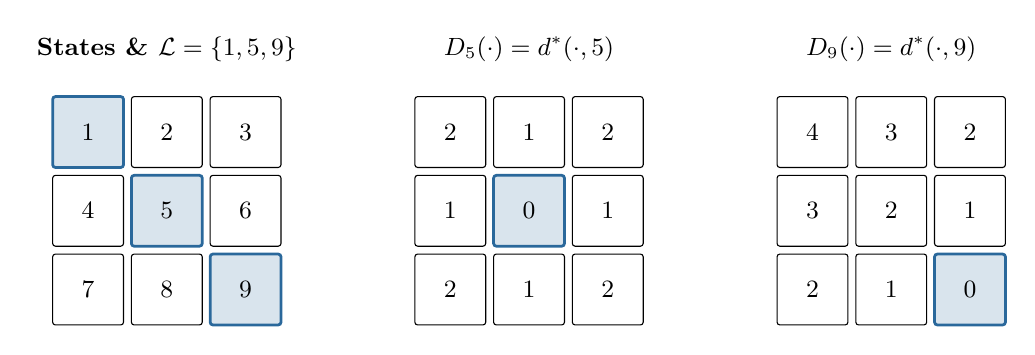
\begin{tikzpicture}[x=1.0cm,y=1.0cm]
  \node[font=\bfseries\small] at (1,1.05) {States \& $\mathcal L=\{1,5,9\}$};
  \foreach \c/\r/\val in {1/0/2, 2/0/3, 0/1/4, 2/1/6, 0/2/7, 1/2/8}{\node[gcell] at (\c,-\r) {\val};}
  \node[lcell] at (0,0) {1}; \node[lcell] at (1,-1) {5}; \node[lcell] at (2,-2) {9};
  \begin{scope}[xshift=4.6cm]
  \node[font=\bfseries\small] at (1,1.05) {$D_5(\cdot)=d^{*}(\cdot,5)$};
  \foreach \c/\r/\val in {0/0/2, 1/0/1, 2/0/2, 0/1/1, 2/1/1, 0/2/2, 1/2/1, 2/2/2}{\node[gcell] at (\c,-\r) {\val};}
  \node[lcell] at (1,-1) {0};
  \end{scope}
  \begin{scope}[xshift=9.2cm]
  \node[font=\bfseries\small] at (1,1.05) {$D_9(\cdot)=d^{*}(\cdot,9)$};
  \foreach \c/\r/\val in {0/0/4, 1/0/3, 2/0/2, 0/1/3, 1/1/2, 2/1/1, 0/2/2, 1/2/1}{\node[gcell] at (\c,-\r) {\val};}
  \node[lcell] at (2,-2) {0};
  \end{scope}
\end{tikzpicture}
\caption{Distance is a lookup table; each cell shows $d^{*}(\text{cell},\ell)$. The same
fields give the membership prior \eqref{eq:membership-prior}: by default a state joins its
nearest landmark.}
\label{fig:fields}
\end{figure}

\section{What is stored, and what is hidden}
\label{sec:hidden}

\begin{table}[htbp]
\centering
\small
\begin{tabularx}{\textwidth}{lllY}
\toprule
Family & Primitive (abstracted) & Latent assignment $z$ & Static representation $\mathcal R_M$ \\
\midrule
Primitive & action & none (degenerate) & $\varnothing$ \\
Action chunk & action \emph{edges} (sequences) & $z^{g}_{n,t}$, per-occurrence parse \emph{(dynamic)} &
grammar $\mathcal G$ (productions over actions) \\
Landmark option & state \emph{nodes} & $z^{\ell}(s)\in\mathcal L$, membership \emph{(static)} &
$(z^{\ell},\mathcal E^{\mathcal L})$: state$\to$region map and region graph \\
\bottomrule
\end{tabularx}
\caption{The two axes of difference. We reserve $z$ for the latent assignment that lifts a
primitive to the abstract layer. There is no separate token $o$: a landmark ``option''
$\ell_i\!\to\!\ell_j$ is a transition between membership values, permitted iff
$(\ell_i,\ell_j)\in\mathcal E^{\mathcal L}$, so the connection lives in the structure, not in
an extra latent.}
\label{tab:hidden}
\end{table}

\textbf{Segmentation is a derived time series.} Once $z$ is fixed, the trajectory splits
into runs of constant assignment. We mark these by a change-point process
\begin{equation}
\chi_{n,t}=\mathbf 1[\,z_{n,t}\neq z_{n,t-1}\,]\in\{0,1\},
\label{eq:changepoint}
\end{equation}
which induces segment boundaries $(u_{n,m},v_{n,m})$, observed runs
$\sigma_{n,m}:=\tau_{n,u_{n,m}:v_{n,m}}$, and durations $\delta_{n,m}=v_{n,m}-u_{n,m}$. For
the landmark family this is fully determined by the static membership and the observed path:
$\chi^{\ell}_{n,t}=\mathbf 1[\,z^{\ell}(s_{n,t})\neq z^{\ell}(s_{n,t-1})\,]$ flags a
region crossing. Thus $\chi$ is bookkeeping, not an extra latent, and $z$ alone carries the
hidden content.

\section{The unified generative graphical model}

\begin{figure}[htbp]
\centering
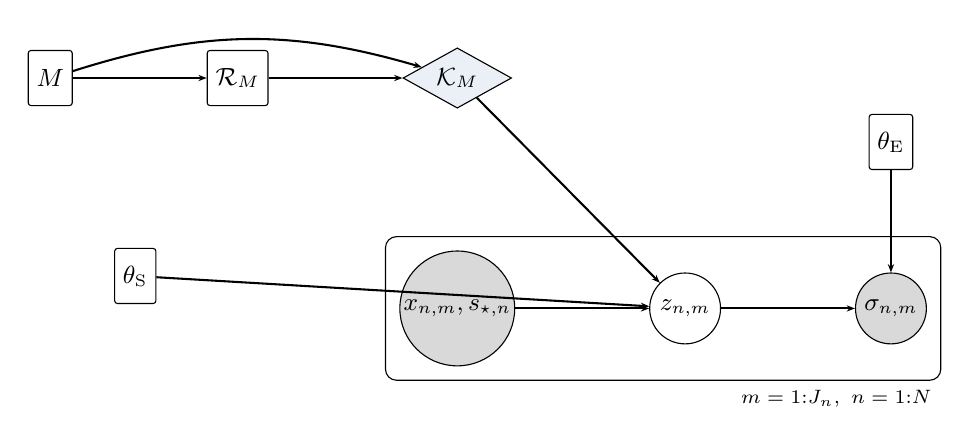
\begin{tikzpicture}[node distance=13mm and 17mm]
  \node[pgm parameter] (M) {$M$};
  \node[pgm parameter,right=of M] (R) {$\mathcal R_M$};
  \node[pgm map,right=of R] (K) {$\mathcal K_M$};
  \node[pgm parameter,below=18mm of R,xshift=-13mm] (thetaS) {$\theta_{\mathrm S}$};
  \node[pgm observed,below=18mm of K] (x) {$x_{n,m},s_{\star,n}$};
  \node[pgm latent,right=of x] (z) {$z_{n,m}$};
  \node[pgm observed,right=of z] (sig) {$\sigma_{n,m}$};
  \node[pgm parameter,above=of sig] (thetaE) {$\theta_{\mathrm E}$};
  \draw[pgm arrow] (M) -- (R);
  \draw[pgm arrow] (M) to[bend left=17] (K);
  \draw[pgm arrow] (R) -- (K);
  \draw[pgm arrow] (K) -- (z);
  \draw[pgm arrow] (thetaS) -- (z);
  \draw[pgm arrow] (x) -- (z);
  \draw[pgm arrow] (z) -- (sig);
  \draw[pgm arrow] (thetaE) -- (sig);
  \node[pgm plate,fit=(x)(z)(sig),
        label={[font=\scriptsize,anchor=north east]south east:$m=1{:}J_n,\ n=1{:}N$}] {};
\end{tikzpicture}
\caption{Unified generative PGM. $z_{n,m}$ is the per-segment value of the latent assignment
($z^{g}$ for chunks, $z^{\ell}$ for landmarks); shaded nodes are observed conditional on the
segmentation $\chi$. The map $\mathcal K_M=F_M(\mathcal K_0,\mathcal R_M)$ is deterministic.}
\label{fig:pgm}
\end{figure}

The family-specific token support at planning node $x$ is
\begin{equation}
\mathcal Z_{\mathrm{primitive}}(x)=\mathcal A(x),\quad
\mathcal Z_{\mathrm{option}}(x)=\mathcal A(x)\cup\mathcal G(x),\quad
\mathcal Z_{\mathrm{landmark}}(x)=\mathcal A(x)\cup\{\ell_j:(z^{\ell}(x),\ell_j)\in\mathcal E^{\mathcal L}\}.
\label{eq:support}
\end{equation}

\section{Search and execution: how a representation generates behavior}
\label{sec:search}

For $z\in\mathcal Z_M(x)$ the stochastic search kernel is the softmax of a search score
$S_M$,
\begin{equation}
p_{\mathrm S}(z\mid x,s_\star,\mathcal K_M,\theta_{\mathrm S})
=\frac{\exp\{S_M(x,z,s_\star;\omega_M,\theta_{\mathrm S})\}}
{\sum_{v\in\mathcal Z_M(x)}\exp\{S_M(x,v,s_\star;\omega_M,\theta_{\mathrm S})\}}.
\label{eq:kernel}
\end{equation}
The simplest concrete, admissible choice of $S_M$ exposes the two roles of $d^{*}$.

\begin{center}
\fbox{\begin{minipage}{0.9\textwidth}
\textbf{Rule 1 --- which landmark to head for (the goal enters here).} At a region boundary
$x=\ell_i$, score each permitted next region by estimated cost-to-goal through it,
\[
S_M(\ell_i,\ell_j,s_\star)=-\beta\bigl[\,d^{*}(\ell_i,\ell_j)+d^{*}(\ell_j,s_\star)\,\bigr],
\qquad (\ell_i,\ell_j)\in\mathcal E^{\mathcal L}.
\]
\textbf{Rule 2 --- which action to take (the target landmark enters here).} While bound for
$\ell_j$, descend its field, $p_{\mathrm E}(a\mid s,\ell_j)\propto\exp\{-\eta\,d^{*}(s'(s,a),\ell_j)\}$,
stopping at the first hit of $\ell_j$.
\end{minipage}}
\end{center}

Both choices read the same field against different targets:
$\widehat d(x,s_\star)=\min\{d^{*}(x,s_\star),\ \min_j[d^{*}(x,\ell_j)+d^{*}(\ell_j,s_\star)]\}$.
The complete forward process per trial: precompute $D_\ell$; set $x\leftarrow s_0$; while
$x\neq s_\star$, pick the next region by Rule 1 and execute toward it by Rule 2. Response
time can be linked to expansions without changing the choice model,
$\log\mathrm{RT}_n\sim\mathcal N(\alpha+\rho\,N_{\mathrm{expand}}(\mathcal K_M,s_{n,0},s_{\star,n}),\nu_{\mathrm{RT}})$.

\section{Complete-data likelihood and joint distribution}

With $\Theta_M=(\theta_{\mathrm S},\theta_{\mathrm E})$, segmenting $\tau_n$ by the
change-points $\chi_n$ into runs $m=1{:}J_n$ gives
\begin{equation}
\boxed{\;
p(\tau_n,z_n\mid M,\mathcal R_M,\Theta_M)
=\prod_{m=1}^{J_n}
p_{\mathrm S}(z_{n,m}\mid x_{n,m},s_{\star,n},\mathcal K_M,\theta_{\mathrm S})\,
p_{\mathrm E}(\sigma_{n,m}\mid z_{n,m},\theta_{\mathrm E},\mathcal K_0)\;}.
\label{eq:like}
\end{equation}
For the primitive family $J_n=T_n$. For the chunk family the latent is the per-occurrence
parse $z^{g}$ and $p_{\mathrm E}$ concentrates on $g$'s action string. For the landmark
family the latent is the static membership $z^{\ell}$: the run labels are the regions
$z^{\ell}(s_{n,t})$, and $p_{\mathrm E}$ is the target-directed kernel of Rule 2; the
representation prior is $p(\mathcal R_M\mid M)=p(z^{\ell})\,p(\mathcal E^{\mathcal L})$ with
$p(z^{\ell})$ from \eqref{eq:membership-prior}. The joint is
\begin{equation}
p(D,z,\mathcal R_M,\Theta_M\mid M)
=p(\mathcal R_M\mid M)\,p(\Theta_M\mid M)\,
\mathbf 1[\mathcal K_M=F_M(\mathcal K_0,\mathcal R_M)]\,
\textstyle\prod_n p(\tau_n,z_n\mid M,\mathcal R_M,\Theta_M).
\label{eq:joint}
\end{equation}
Exact inference sums over memberships, grammars, and parses and is infeasible, motivating the
Bayesian structural EM of Analysis 8.

\section{A worked example, end to end}

Take $\mathcal L=\{1,5,9\}$ with region links
$\mathcal E^{\mathcal L}\supseteq\{(1,5),(5,9)\}$ and read distances from
Figure~\ref{fig:fields}. \emph{(a)} From region $1$ to goal $9$: the scores of
$(1,5)$ and the two primitive steps tie at $4$; a prior preferring fewer decisions selects
the region link --- the point of abstraction. \emph{(b)} Same start, goal $3$: the primitive
step wins ($2<4$); the centre landmark leads away. \emph{(c)} From region $5$ with links
$(5,1),(5,9)$: goal $9$ picks $(5,9)$, goal $1$ picks $(5,1)$ --- the goal selects the
region. \emph{(d)} Two routes $1\!\to\!2\!\to\!5$ and $1\!\to\!4\!\to\!5$ both descend
$D_5$, so they are different realizations of the same region transition. By the triangle
inequality a region link is never shorter than going direct on a uniform grid; its value is
the reusable static abstraction and the cheap distance estimate, and it shortens a path only
when $\mathcal E^{\mathcal L}$ stores a genuine shortcut.

\section{Summary}

The generative model is one chain \eqref{eq:hierarchy}: a static representation
$\mathcal R_M$, an induced map $\mathcal K_M$, a latent assignment $z$, and an observed
trajectory $\tau_n$ whose segmentation $\chi$ is derived. The families differ by what they
abstract --- action edges into a grammar $\mathcal G$ with a dynamic parse $z^{g}$, or state
nodes into a static membership $z^{\ell}$ with a region graph $\mathcal E^{\mathcal L}$
(Figure~\ref{fig:overview}). Recovering these representations by Bayesian structural EM is
Analysis 8.

\end{document}
